%%%%%%%5 PAD MULTI %%%%%%%%%%%%%%
\chapter{PAD multi-ataque y multi-sensor}\label{ch:PAD_MULTIATAQUE}

Existen muchos estudios que presentan diferente métodos para hacer frente a ataques de presentación pero la mayoría de ellos consideran sólo un numero limitado de tipos de ataque y un único sensor de captura.

En este capítulo se hace un análisis de los distintos métodos presentados en la literatura pero considerando distintos tipos de ataque de forma aislada y en conjunto. Además se evalúan también en capturas realizadas con diferentes sensores. Los ataques y los sensores considerados son los incluidos en la base de datos \textit{\Gls{FRAV-Attack}} presentada en la Sección \ref{subsec:FRAV-ABC-ATTACK}.

El objetivo es implementar un mecanismo de PAD que ofrezca una solución global para sistemas \GLS{ABC}, capaz de hacer frente a todas las posibles amenazas de ataques directos al sistema de captura.


Primero evaluamos cada uno de los algoritmos propuestos en la literatura para distintos ataques con todos los ataques considerados en \textit{\gls{FRAV-Attack}},


Como el sistema debe hacer frente a los distintos ataques contemplados se plantea una solución milimétrica con fusión a nivel \textit{scores} (Como se ve en la gráfica se consigue un mejor resultado en la fusión de \GLS{PAD} para cada tipo de ataque que un \GLS{PAD} para detectar todos los ataques en conjunto).

Los algoritmos se pueden agrupar en dos conjuntos 

\color{blue}La primera versión de este \GLS{PAD} se ha entrenado con imágenes de una base de datos construida en un laboratorio \textit{\Gls{FRAV-Attack}} que incluye tanto imágenes \gls{bona-fide} como imágenes con presentaciones de ataques con los \GLSpl{PAI} más comunes en la literatura (para ver más información sobre esta base de datos ver Sección \ref{sec:BBDD-FRAV-Attack}).\color{black}

%%%%%%%5 PREPROCESADO %%%%%%%%%%%%%%
\section{Preprocesado}\label{sec:PAD_PRERPROCESADO}

\begin{figure}
\centering
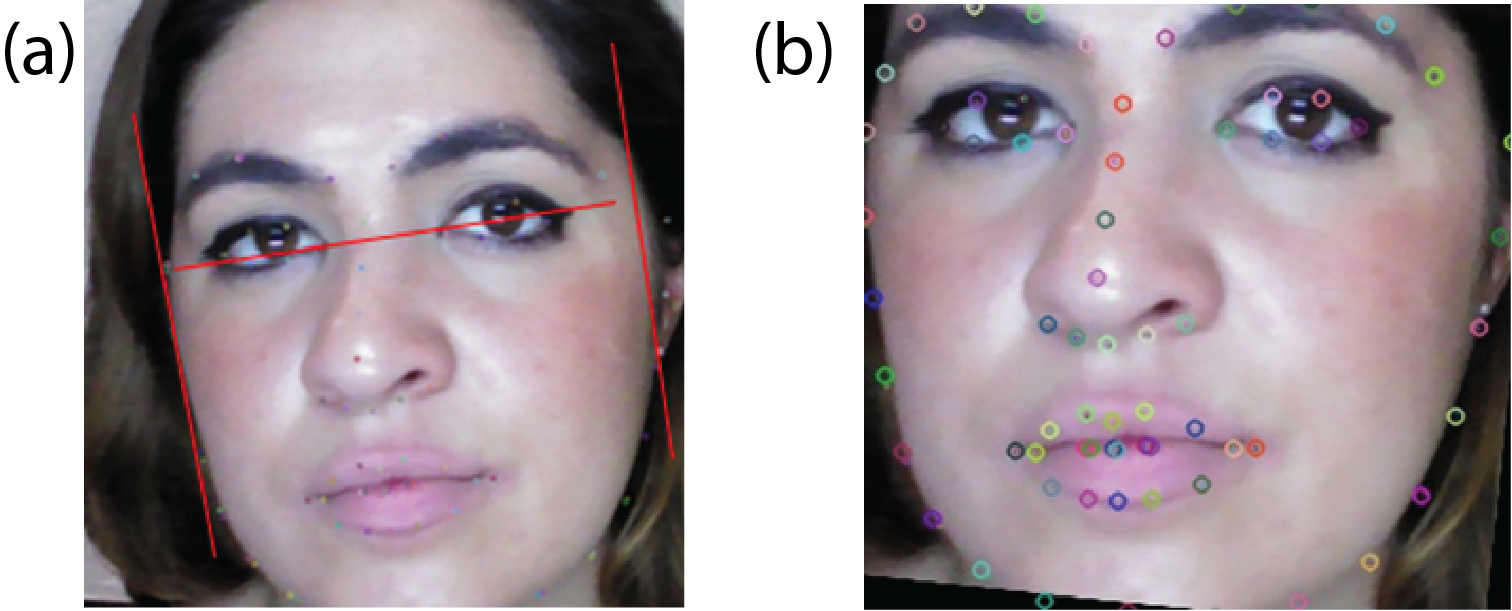
\includegraphics[width=1\textwidth]{ch-sistemasABC/images/ch-evaluacion_topologias/CORRECION_DE_POSE.png}
    \caption{Corrección de la pose de la cara.}
    \label{fig:CORRECCION_DE_LA_POSE}
\end{figure}

Se ajusta la cara atendiendo a la región delimitada por los \textit{landmarks} y se corrigen las posibles inclinaciones atendiendo a los \textit{landmark} de los ojos (Figura \ref{fig:CORRECCION_DE_LA_POSE}).

Con estos ajustes se ejecutan clasificaciones anteriores y se comparan los resultados para verificar si mejoran con el ajuste.

Para ello se ha seleccionado un tercio de la imágenes para entrenar la \GLS{SVM} y el resto para verificar los resultados. 

\textbf{Comparación de la clasificación con nube densa de profundidades} (Fig. X).

% \begin{figure}
% \centering
% 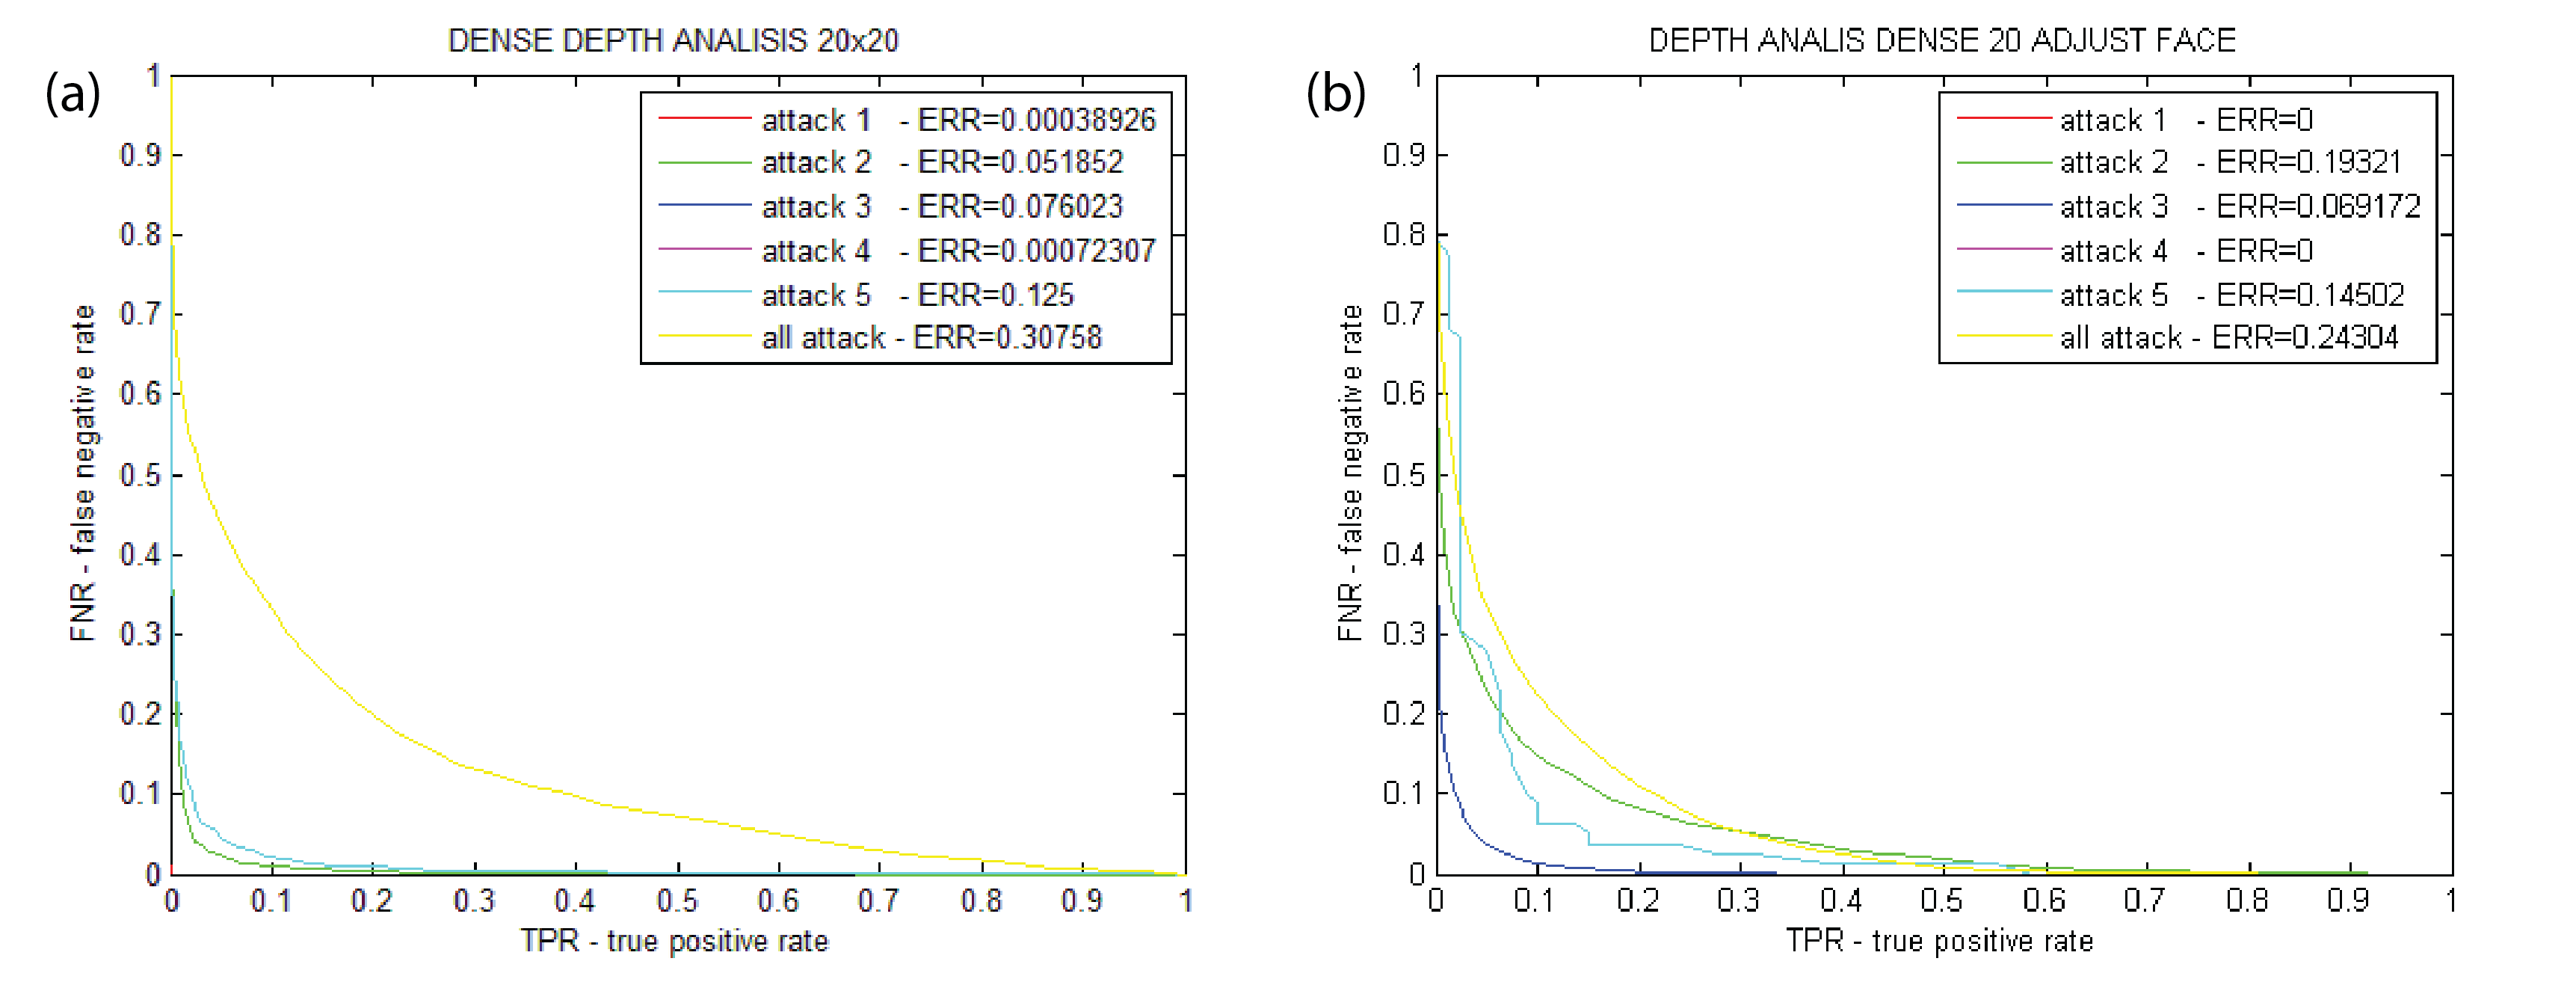
\includegraphics[width=1\textwidth]{ch-sistemasABC/images/ch-evaluacion_topologias/COMPARACION_DESA.png}
%     \caption{Comparación de los resultados considerando una nube densa de puntos, con corrección y sin corrección de la pose.}
%     \label{fig:COMPARACION_DENSA}
% \end{figure}

\textbf{Comparación de la clasificación con histogramas de profundidad por regiones}  (Fig, X). 
% \begin{figure}
% \centering
% 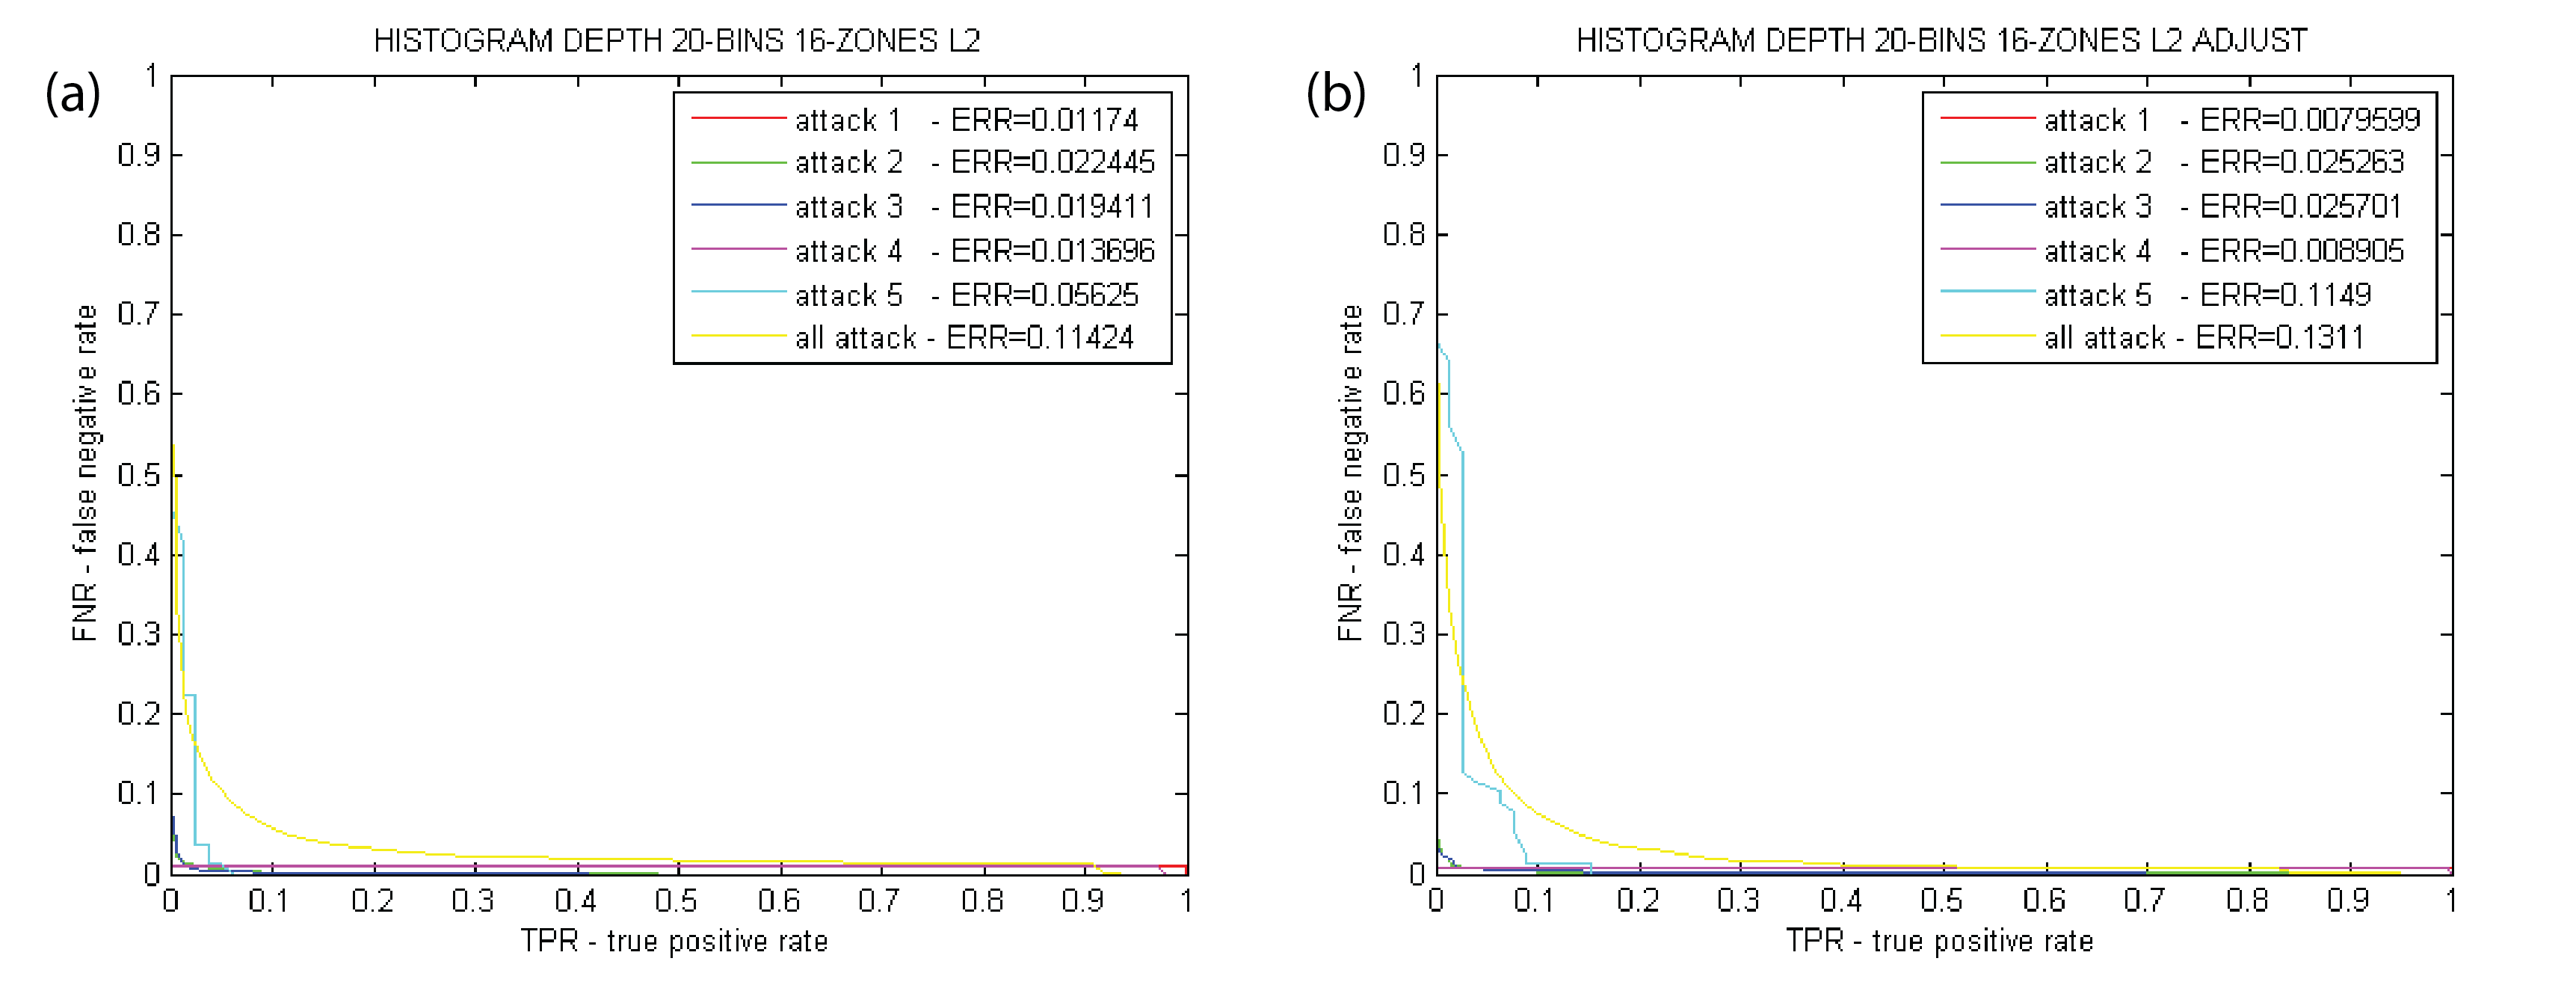
\includegraphics[width=1\textwidth]{ch-sistemasABC/images/ch-evaluacion_topologias/COMPARACION_HISTOGRAMA_REGIONES.png}
%     \caption{Comparación de los resultados considerando los histogramas por regiones, con corrección y sin corrección de la pose.}
%     \label{fig:COMPARACION_HISGRAMA_REGIONES}
% \end{figure}

%%%%%%%5 PAD BASADOS EN TEXTURAS %%%%%%%%%%%%%%
\section{Algoritmos basados en texturas}\label{sec:PAD_TEXTURAS}

\paragraph{\textbf{Clasificación basada en \textit{Depth} calculando \GLS{LBP}}}

Se calcula el \GLS{LBP} de las imágenes de profundidad. (Fig. x).

% \begin{figure}
% \centering
% 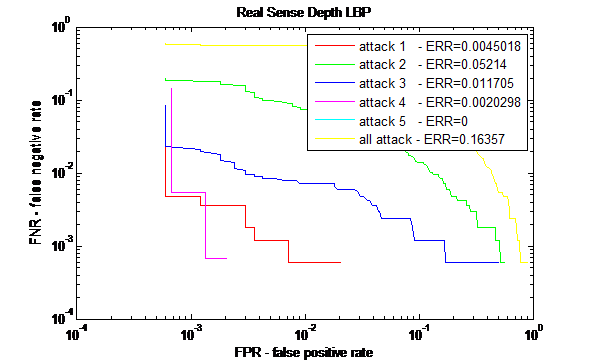
\includegraphics{ch-sistemasABC/images/ch-evaluacion_topologias/DET_LBP_PROFUNDIDAD.png}
%     \caption{\GLS{DET} del \GLS{SVM} de con \GLS{LBP} en la imagen de profundidad.}
%     \label{fig:DET_PROFUNDIDAD_LBP}
% \end{figure}

\paragraph{\textbf{Clasificación basada en \GLS{RGB} calculando \GLS{LBP}}}

% \begin{figure}
% \centering
%     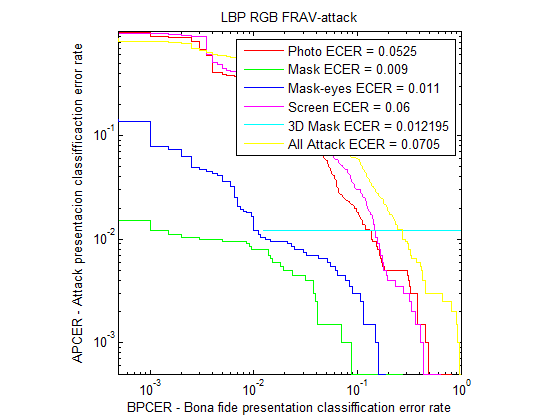
\includegraphics[width=1\textwidth]{ch-sistemasABC/images/ch-evaluacion_topologias/DET_LBP_RGB.png}
%     \caption{\GLS{DET} del \GLS{SVM} de con \GLS{LBP} en la imagen \GLS{RGB}.}
%     \label{fig:DET_RGB_LBP}
% \end{figure}

Se calcula el \GLS{LBP} de las imágenes \GLS{RGB} (Fig. X).

La nueva implementación consiste en localizar la cara con la imagen \GLS{RGB}, segmentarla, reducirla a $100\times100$ y calcular el histograma \GLS{LBP} con \GLS{OpenCV}.

Entrenar un \GLS{SVM} biclase con cada ataque frente a un usuario real. Y también una \GLS{SVM} con todos los ataques agrupados frente a un usuario real.

\color{black}

Los experimentos presentados este capitulo fueron realizados durante la implantación de los dispositivos pilotos del proyecto \GLS{ABC4EU} \cite{ABC4EUOnline}, del Séptimo Programa Marco de la \GLS{EU}. Los resultados obtenidos en dichos experimentos y las conclusiones extraídas se exponen en detalle en la sección \ref{sec:ResultadosABC4EU}. 

Experimentos en un entorno real (Aeropuerto Adolfo Suarez Madrid-Barajas \cite{aeropuertoMadridBarajas}) para evaluar y comparar el rendimiento de sistemas \GLS{ABC} con distintas topologías. 

El presente capitulo describe el piloto de un sistema de control automático de fronteras \GLS{ABC} desarrollado durante el proyecto \GLS{ABC4EU} y que se ajusta a las leyes establecidas para la zona \Gls{Schengen}.

Los dispositivos del sistema \GLS{ABC} analizados tienen una topología \textit{<<Segregated Two Step>>} (para mas información sobre este tipo de sistemas ver Sección \ref{subsec:Topologias}), con una configuración estructural dividida en dos dispositivos: el registro en un \gls{e-kiosk} y la verificación y el cruce de frontera en una \gls{e-gate} de tipo \gls{mantrap}. Esto implica dos etapas de captura y dos puntos sensibles en los que el sistema puede sufrir ataques de presentación. Las pruebas se llevaron a cabo con un piloto del sistema, en la terminal T$4$-S (satélite T$4$) del aeropuerto Adolfo Suárez de Madrid-Barajas, donde se capturó la base de datos \Gls{FRAV-ABC-Attack}.

Los experimentos ponen a prueba la seguridad del sistema simulando diferentes ataques de presentación, ambas etapas del sistema: registro y verificación. Loa ataques contemplados son los incluidos en \Gls{FRAV-ABC-Attack}: Foto, máscara, mascara sin ojos, vídeo, máscara $3$D y camiseta. (ver Sección \ref{subsec:FRAV-ABC-ATTACK}).

Finamente los resultados obtenidos para cada uno de los ataques se presenta en la Sección \ref{sec:ResultadosABC4EU}, indicando aquellos ataques que pueden resultar más peligrosos para el sistema y sugiriendo algunas contramedidas que podrían aumentar la fiabilidad y la seguridad del sistema.

%%%%%%%5 PAD BASADOS EN DESCRIPTORES %%%%%%%%%%%%%%
\section{Algoritmos basados en descriptores}\label{sec:PAD_DESCRIPTORES}

Analizamos la profundidad de imágenes recortadas con la región de la cara de cada fotograma.

Clasificación basada en el análisis de las profundidades de forma densa.

Se analiza una serie de puntos equidistantes distribuidos de forma densa por toda la imagen. De cada punto se toma la profundidad y se compone un vector con los valores de profundidad en cada punto. Estos vectores de características serán con los que entrenaremos la \GLS{SVM}.

Los pasos detallados del algoritmo son:
\begin{enumerate}
\item
Localización de la cara con \Gls{Viola-Jones} en la imagen \GLS{RGB}.

\item
Segmentación de la región de la cara en la matriz de profundidad que está registrada con la imagen \GLS{RGB}.

\item
Normalizamos los valores de profundidad para la región de la cara. Para ello:

Se seleccionan todas las profundidades distintas de $0$. (Las distancias $0$ son aquellas que no han podido ser calculadas por la cámara).

Se calcula la media y la desviación para establecer un límite máximo y mínimo de las profundidades a considerar.

% cv::meanStdDev(cleanDepth, mean, stddev);
% double cleanMin = mean.val[0] - 4 * stddev.val[0];
% double cleanMax = mean.val[0] + 4 * stddev.val[0]; 

Los puntos \textit{outlayers}, es decir los que tiene profundidades fuera de estos límites se establecen a $0$ y el resto de las profundidades se normalizan atendiendo a la profundidad máxima y mínima calculada.

% depthImage.at<float>(row, col) = (1 - ((depthImage.at<float>(row, col) - cleanMin) / (cleanMax - cleanMin))) * 255;

\item
Se reduce la matriz con las profundidades de la cara a un tamaño de $300\times300$.

\item
Se construye un vector con las profundidades de una serie de puntos distribuidos en una rejilla uniforme (por ejemplo, de $10\times10$) sobre la imagen. 

\end{enumerate}

\paragraph{\textbf{Clasificación basada en el análisis de las profundidades de forma densa}}

Imágenes de clasificación basada en el análisis de profundidad de las imágenes analizándola en el punto de interés (Figura \ref{fig:PUNTOS_DE_INTERES_EN_IMAGENES_DE_PROFUNDIDAD} y figura \ref{fig:PUNTOS_DE_INTERES_EN_IMAGENES_DE_PROFUNDIDAD_EN_ATAQUES}).

\begin{figure}
\centering
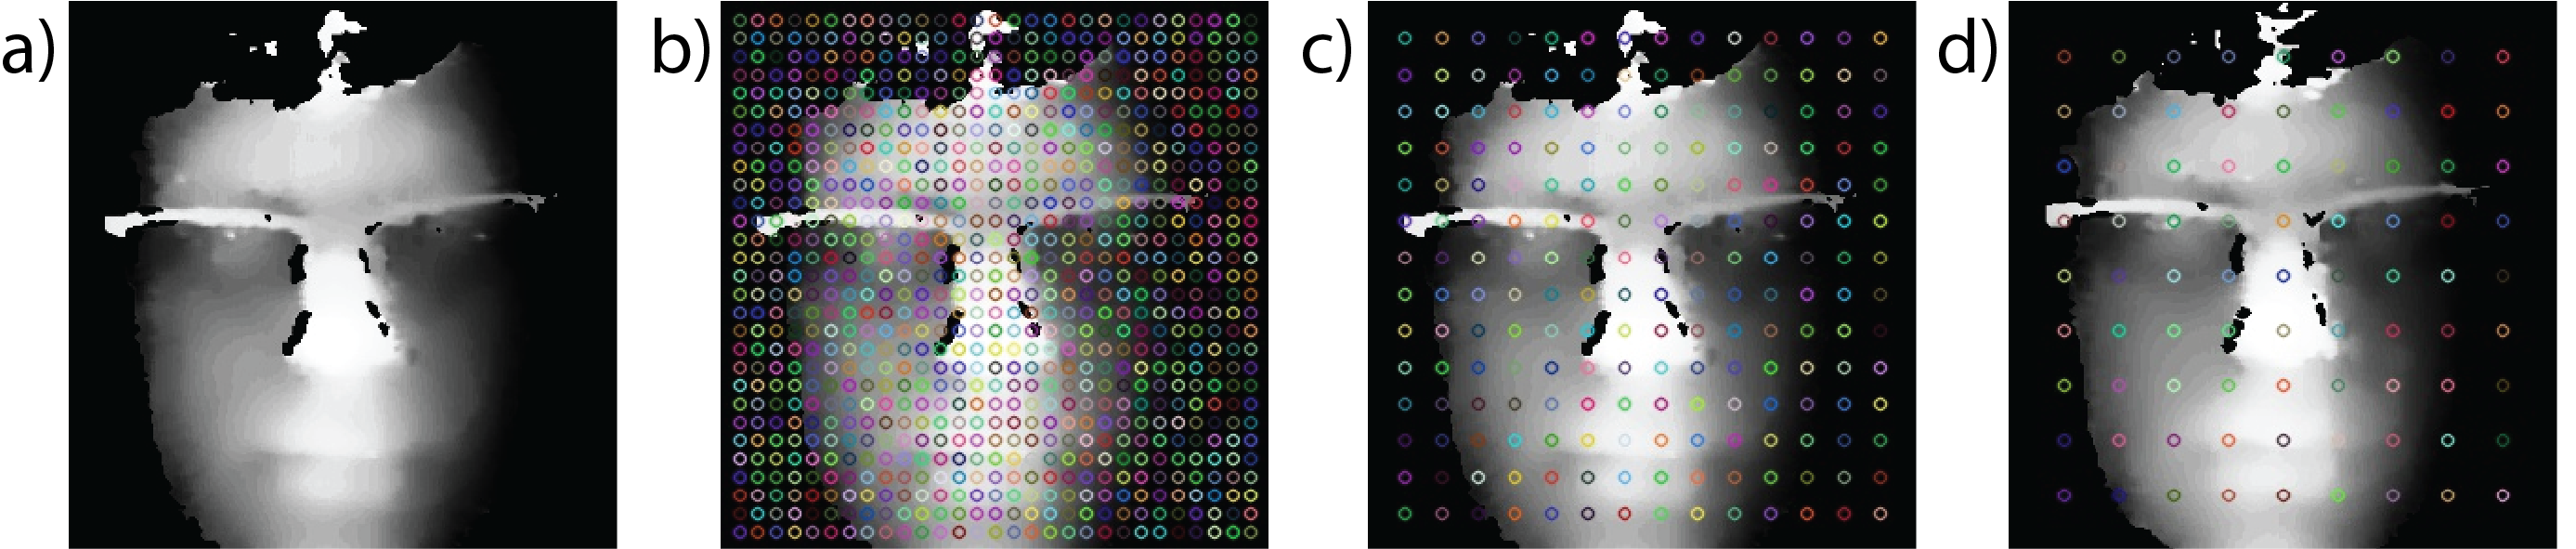
\includegraphics[width=1\textwidth]{ch-sistemasABC/images/ch-evaluacion_topologias/PUNTOS_DE_INTERES_EN_IMGS_PROFUNDIDAD.png}
    \caption{Puntos de interés en imágenes de profundidad.}
    \label{fig:PUNTOS_DE_INTERES_EN_IMAGENES_DE_PROFUNDIDAD}
\end{figure}
 
\begin{figure}
\centering
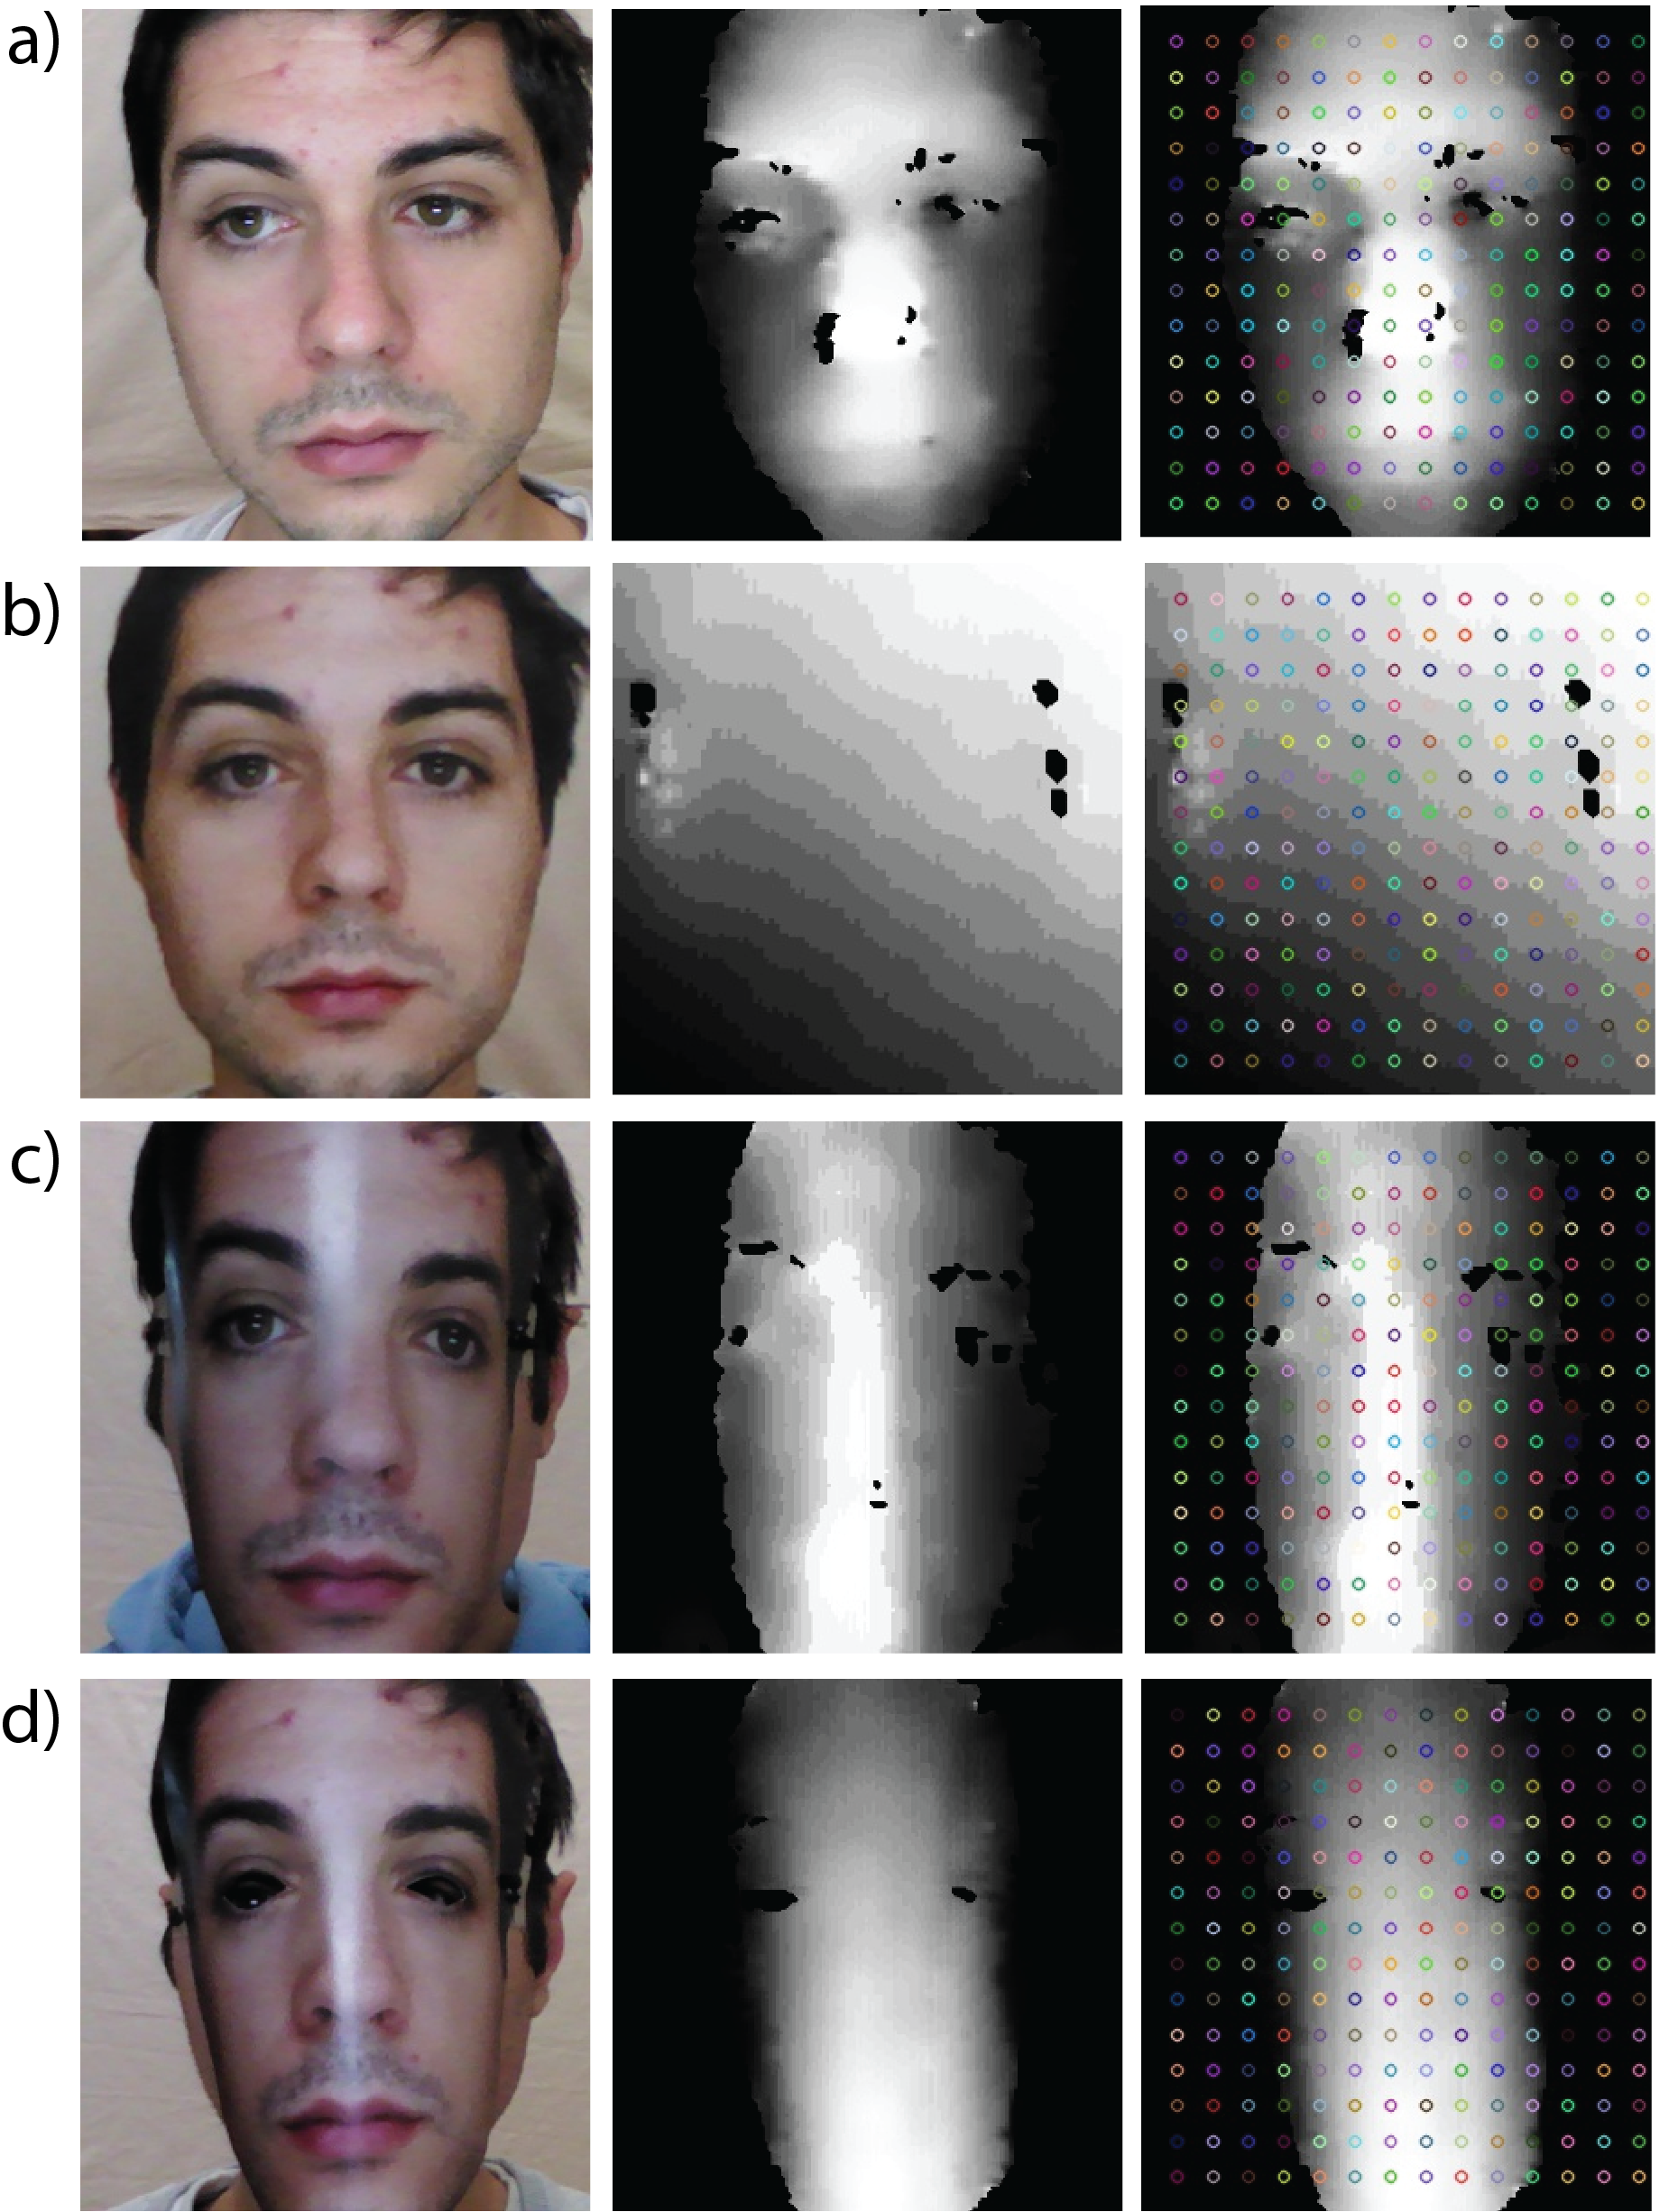
\includegraphics[width=0.6\textwidth]{ch-sistemasABC/images/ch-evaluacion_topologias/PUNTOS_DE_INTERES_EN_IMGS_PROFUNDIDAD_2.png}
    \caption{Puntos de interés en imágenes de profundidad en los distintos ataques de \Gls{FRAV-Attack}.}
    \label{fig:PUNTOS_DE_INTERES_EN_IMAGENES_DE_PROFUNDIDAD_EN_ATAQUES}
\end{figure}

Resultados de clasificación basada en el análisis de profundidad de las imágenes analizándolas con una nube de puntos densa (Figura \ref{fig:RESULTADOS_PROFUNDIDAD_DENSA}).

\begin{figure}
\centering
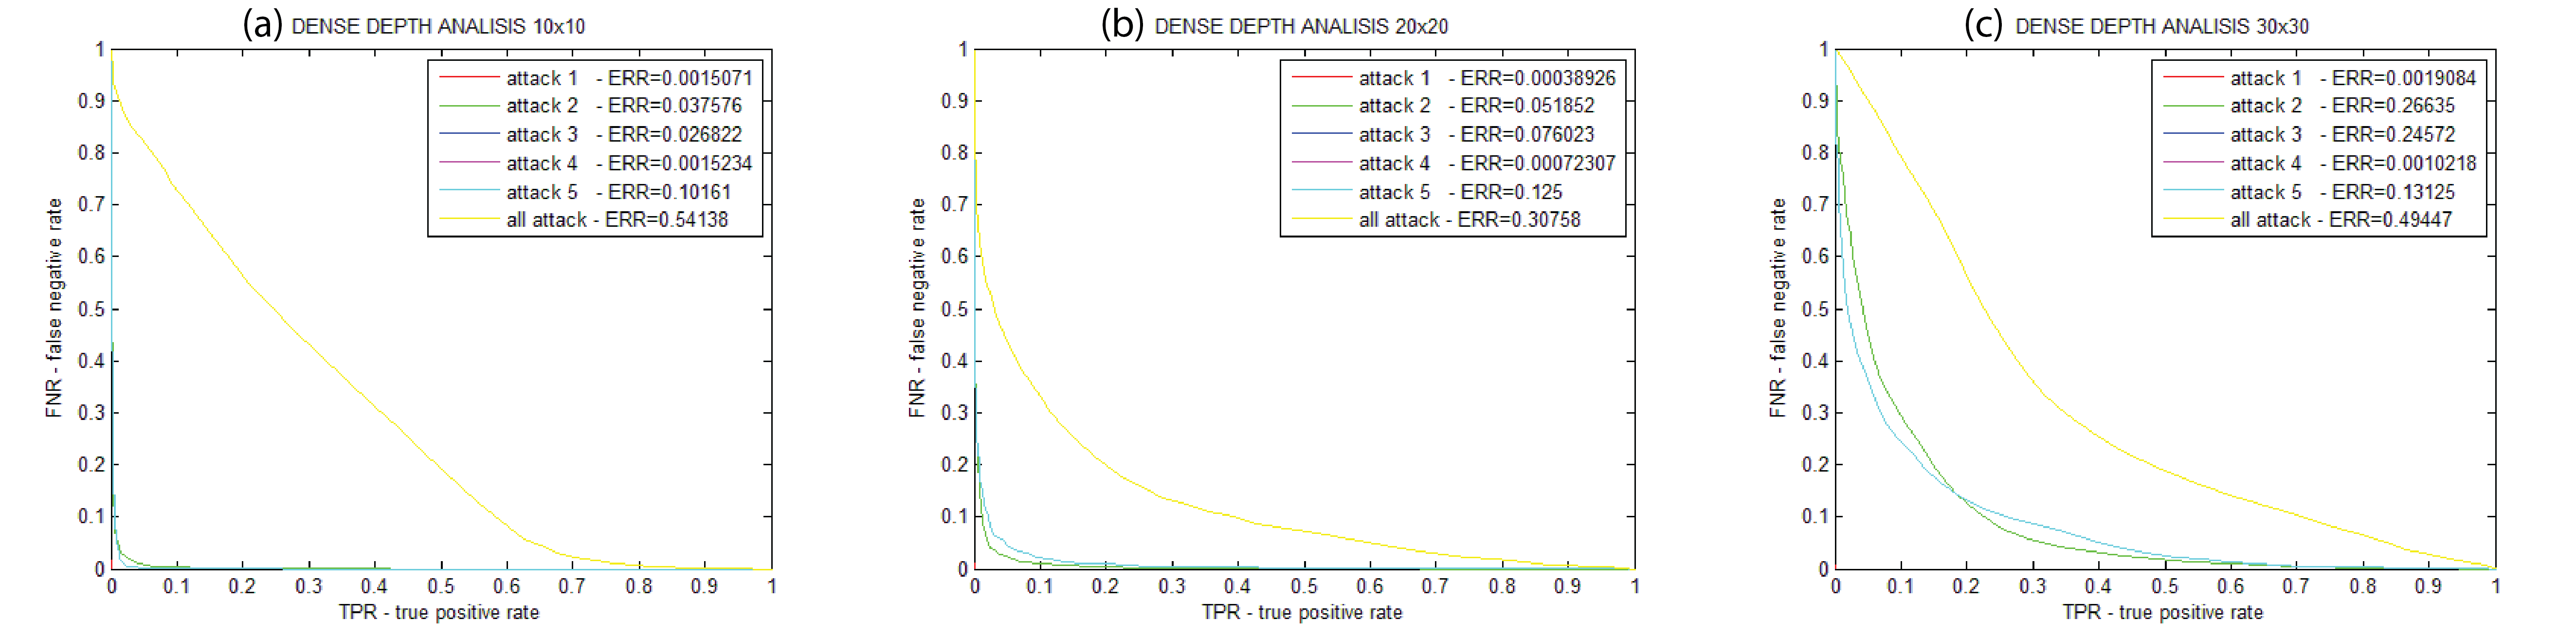
\includegraphics[width=1\textwidth]{ch-sistemasABC/images/ch-evaluacion_topologias/RESULTADOS_PROFUNDIDAD_DENSA.png}
    \caption{Resultados de clasificación basada en el análisis de profundidad de las imágenes analizándolas con una nube de puntos densa.}
    \label{fig:RESULTADOS_PROFUNDIDAD_DENSA}
\end{figure}

\paragraph{\textbf{Clasificación basada en el análisis de las profundidades en puntos de interés}}

Imágenes de clasificación basada en el análisis de profundidad de las imágenes analizándola en el punto de interés (Figura \ref{fig:SIFT_EN_IMAGENES_DE_PROFUNDIDAD_EN_ATAQUES}).

\begin{figure}
\centering
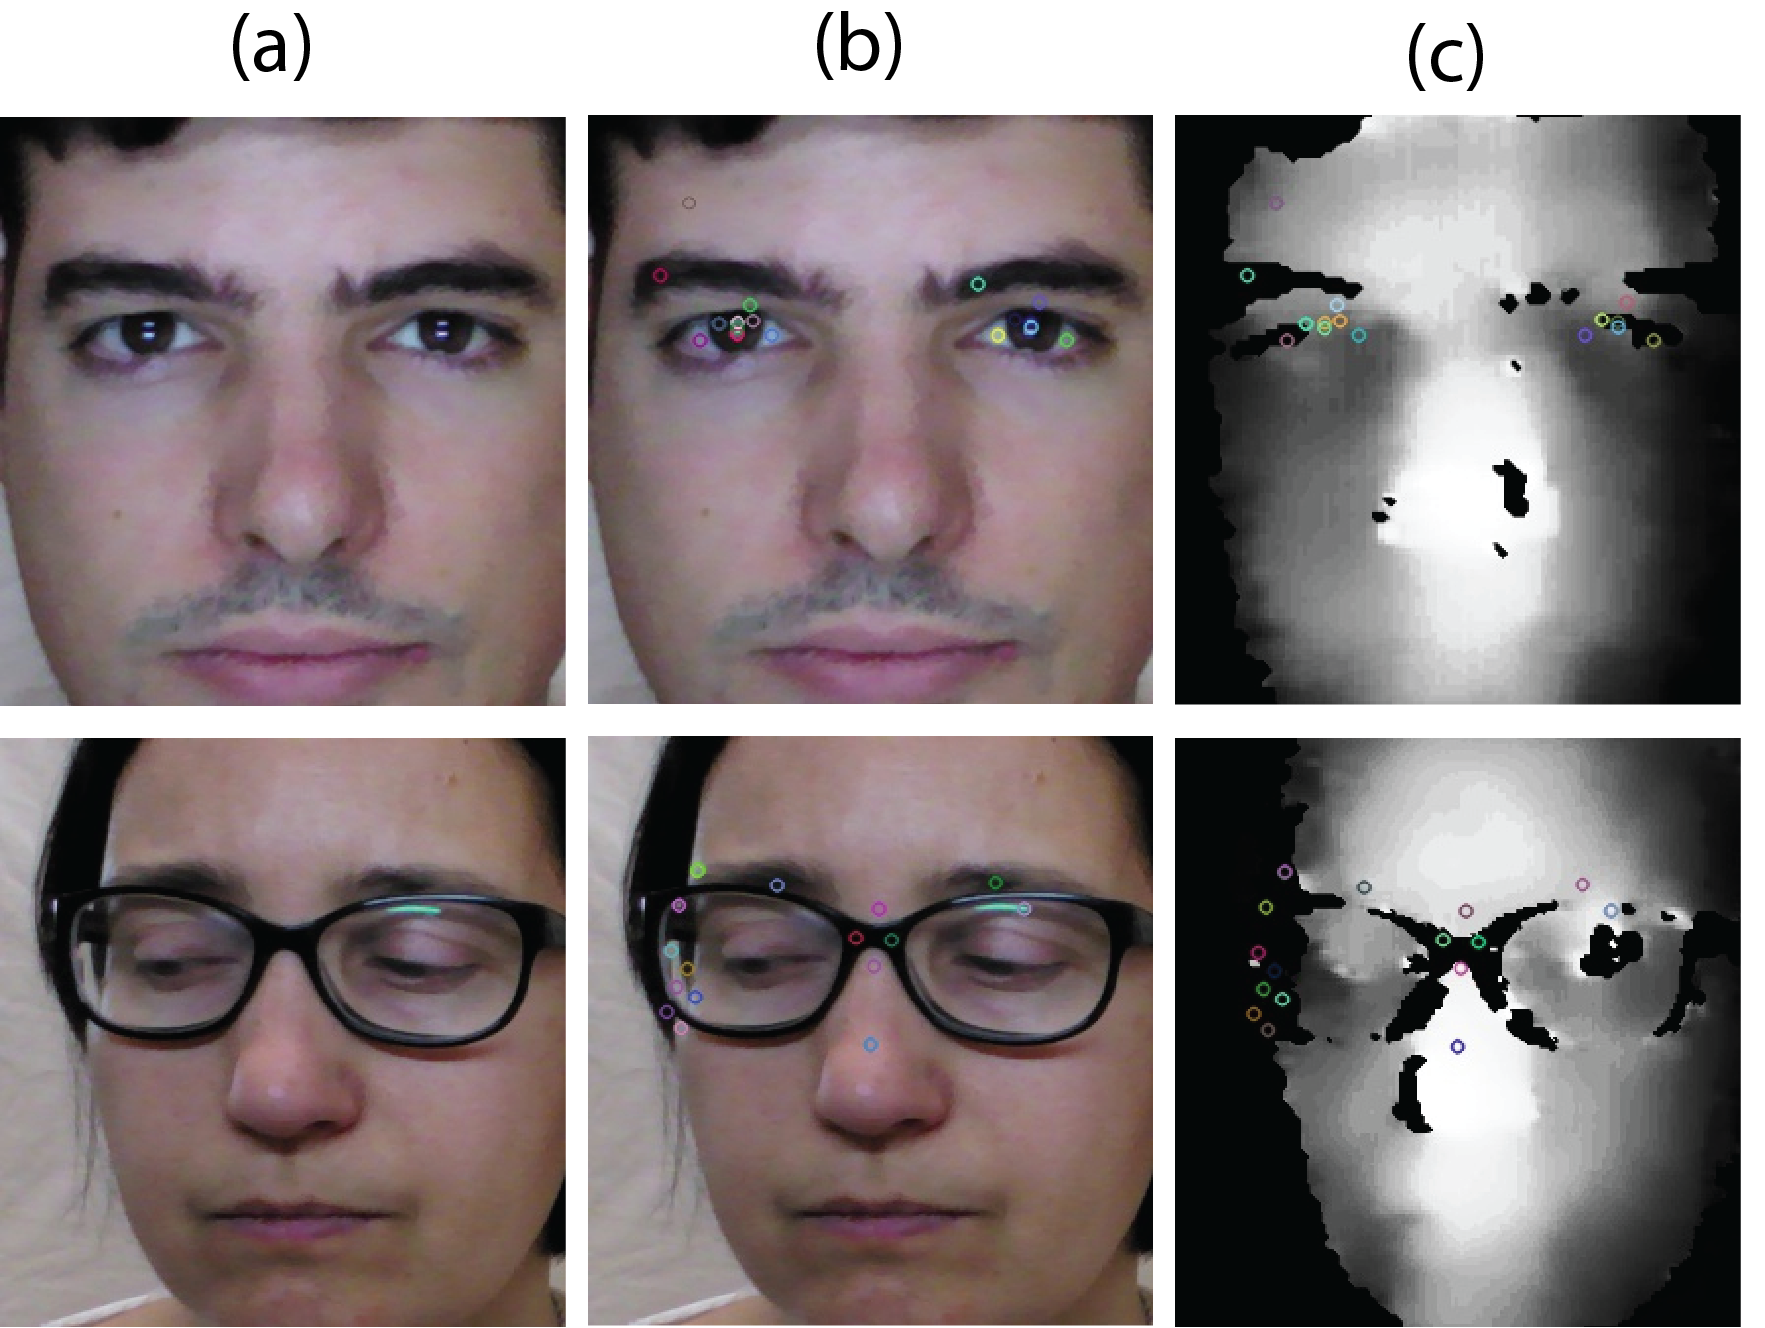
\includegraphics[width=0.6\textwidth]{ch-sistemasABC/images/ch-evaluacion_topologias/SIFT_EN_IMGS_PROFUNDIDAD.png}
    \caption{\gls{SIFT} en imágenes de profundidad en los distintos ataques de \textit{\Gls{FRAV-Attack}}.}
    \label{fig:SIFT_EN_IMAGENES_DE_PROFUNDIDAD_EN_ATAQUES}
\end{figure}

Resultados de clasificación basada en el análisis de profundidad de las imágenes analizándola en el punto de interés (Figura \ref{fig:RESULTADOS_PROFUNDIDAD_SIFT}).

\begin{figure}
\centering
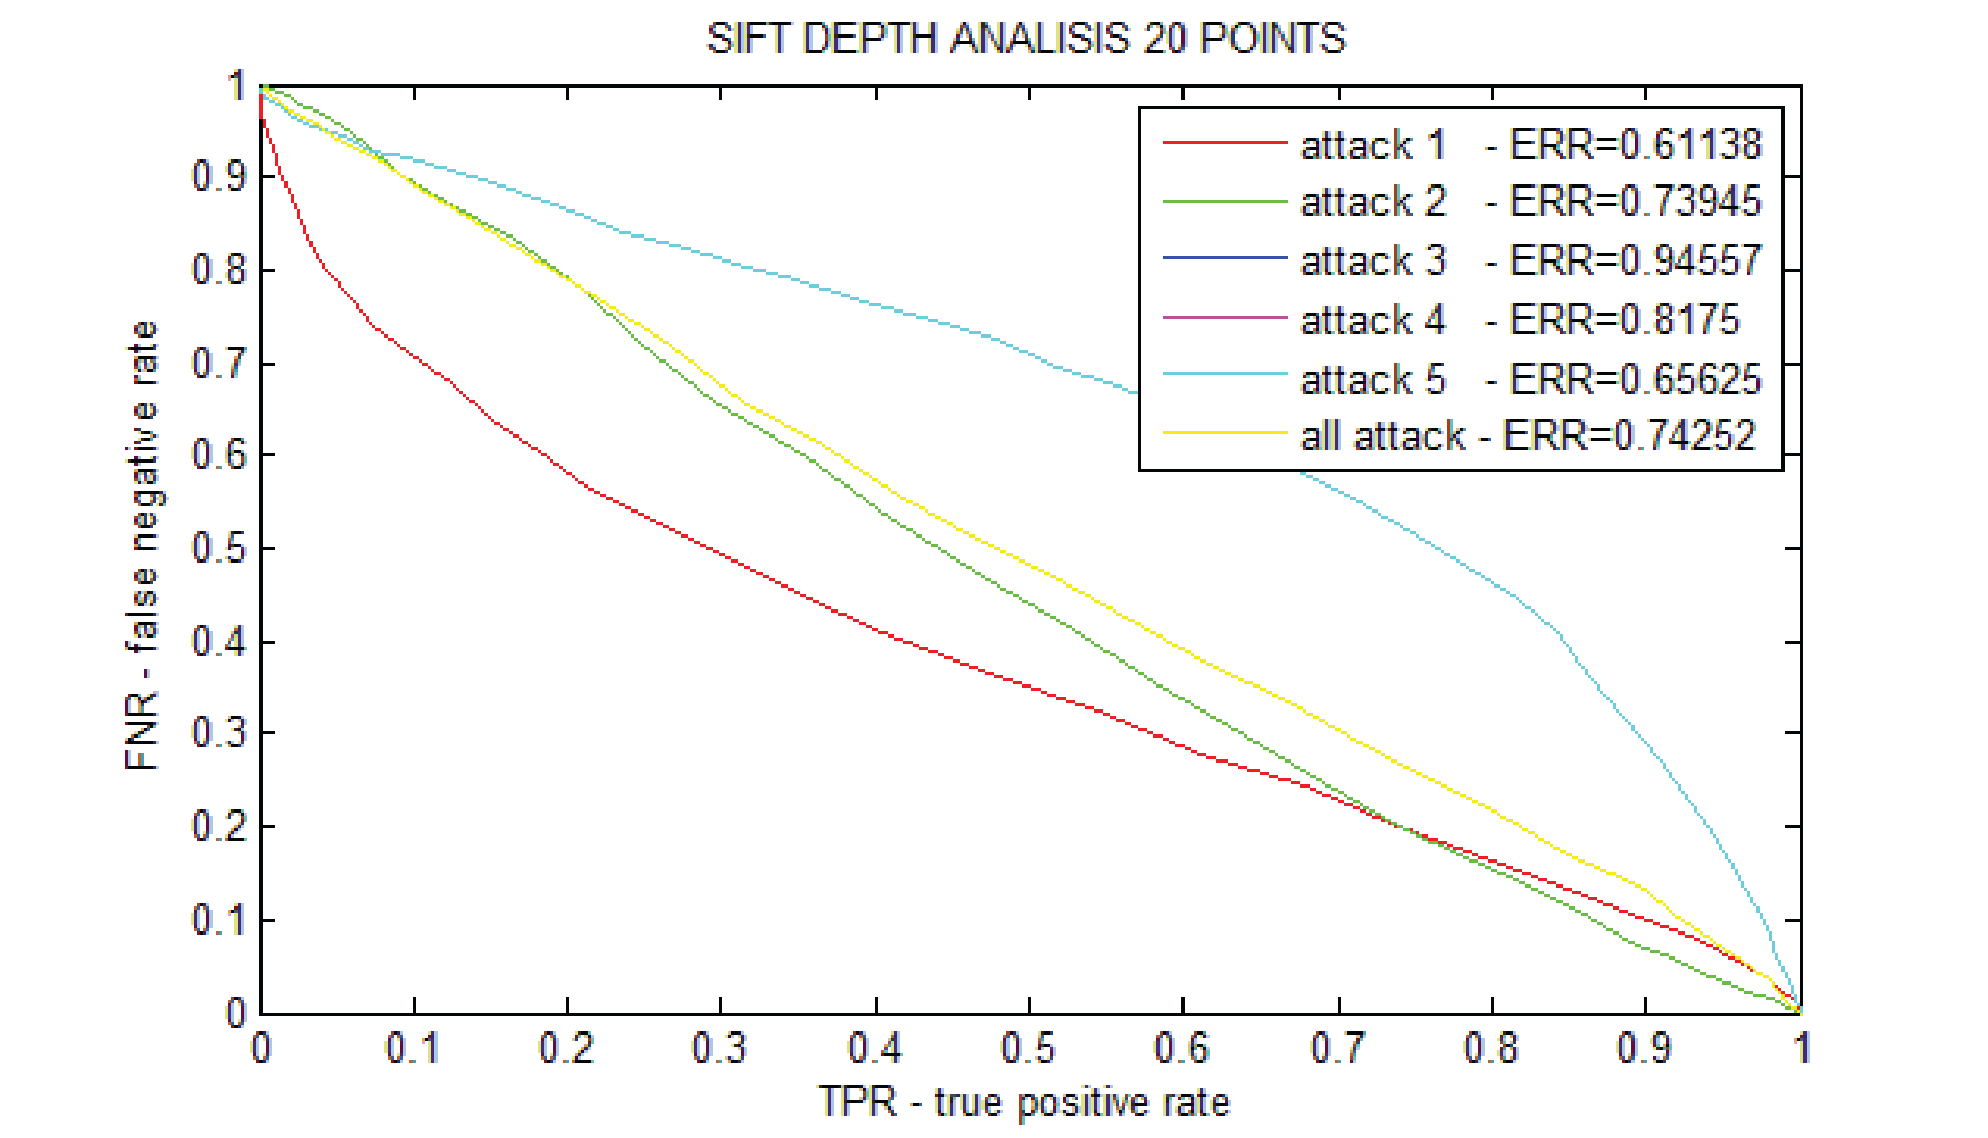
\includegraphics[width=1\textwidth]{ch-sistemasABC/images/ch-evaluacion_topologias/RESULTADOS_PROFUNDIDAD_SIFT.png}
    \caption{Resultados de clasificación basada en el análisis de profundidad de las imágenes analizándola en el punto de interés.}
    \label{fig:RESULTADOS_PROFUNDIDAD_SIFT}
\end{figure}

\paragraph{\textbf{Clasificación basada en los histogramas de profundidad}}

Histogramas obtenidos de las imágenes de profundidad (Figura \ref{fig:HISTOGRAMAS_DE_PROFUNDIDAD}).

\begin{figure}
\centering
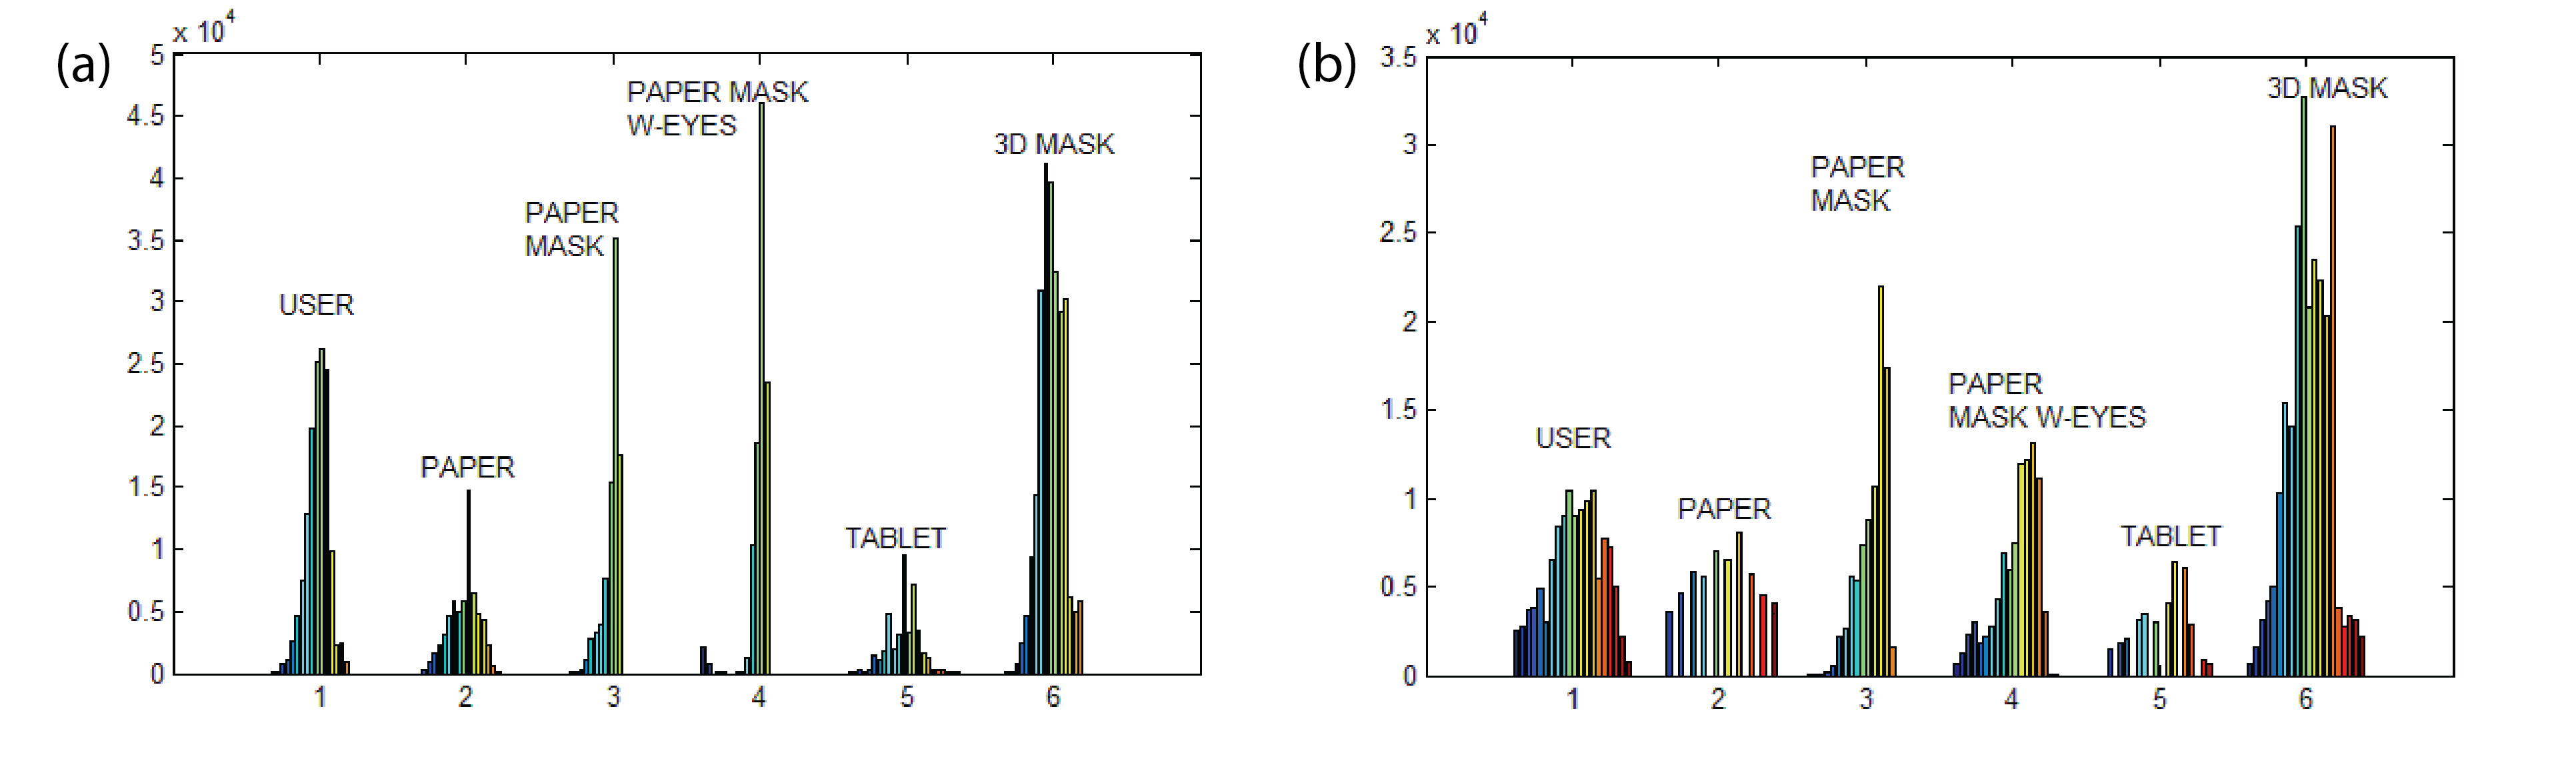
\includegraphics[width=1\textwidth]{ch-sistemasABC/images/ch-evaluacion_topologias/HISTOGRAMAS_DE_PROFUNDIDAD.png}
    \caption{Histogramas de profundidad.}
    \label{fig:HISTOGRAMAS_DE_PROFUNDIDAD}
\end{figure}

Resultados de clasificación basada en el análisis de profundidad de las imágenes analizándola en el punto de interés (Figura \ref{fig:RESULTADOS_HISTOGRAMAS_DE_PROFUNDIDAD}).

\begin{figure}
\centering
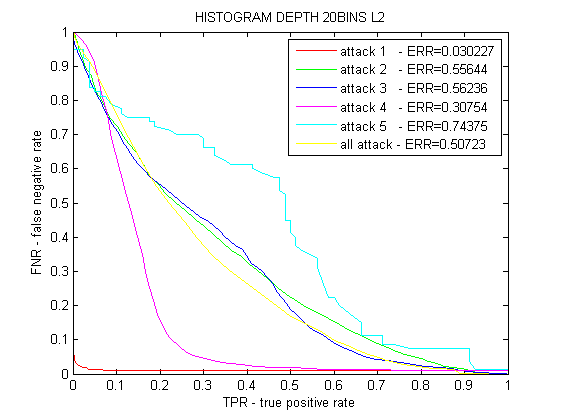
\includegraphics[width=1\textwidth]{ch-sistemasABC/images/ch-evaluacion_topologias/RESULTADOS_CLASIFICACION_POR_HISTROGRAMAS.png}
    \caption{Resultados obtenidos con los histogramas de profundidad.}
    \label{fig:RESULTADOS_HISTOGRAMAS_DE_PROFUNDIDAD}
\end{figure}

\paragraph{\textbf{Clasificación basada en los histogramas de profundidad teniendo en cuenta la información regional ($4$ regiones, $16$ regiones).}}

Se calcula el histograma con $20$ niveles de profundidad de cada una de estas regiones y se concatenan los histogramas.

Considerando $4$ particiones en la imagen y considerando la concatenación de los histogramas de $16$ regiones (Figura \ref{fig:HISTOGRAMAS_POR_REGIONES}).

\begin{figure}
\centering
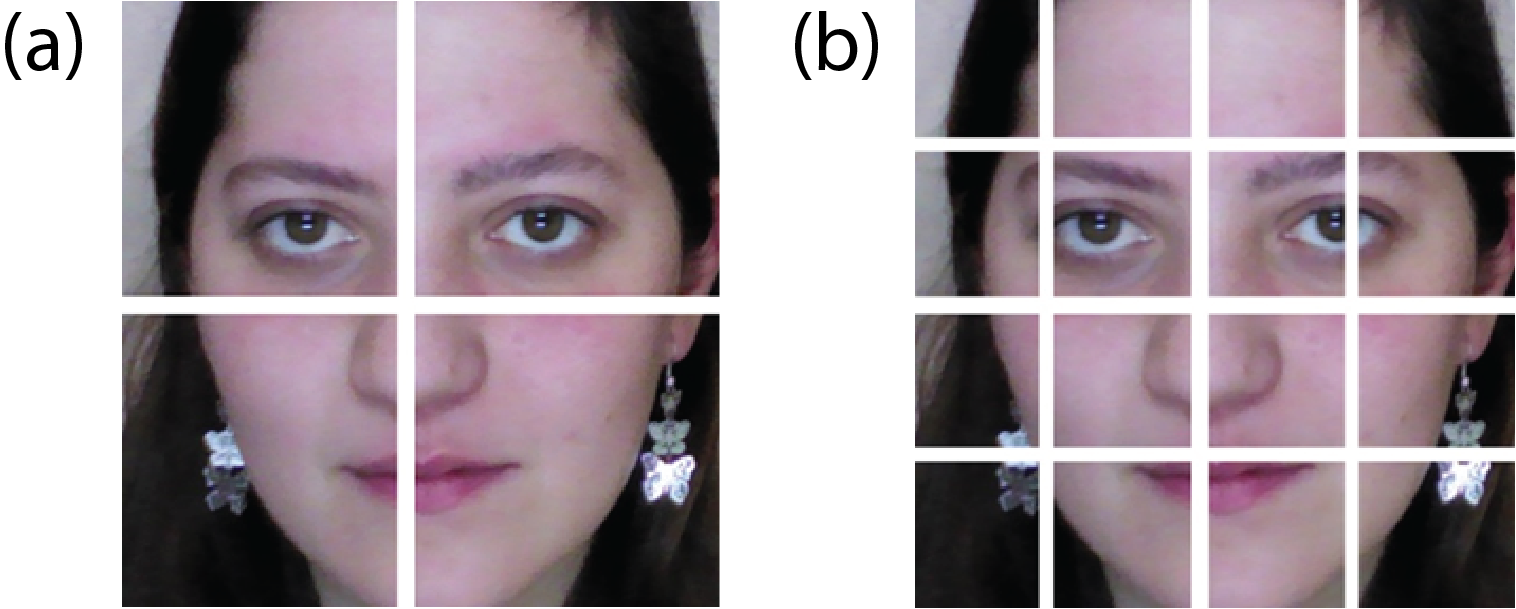
\includegraphics[width=1\textwidth]{ch-sistemasABC/images/ch-evaluacion_topologias/HISTOGRAMAS_ANALIZADOS_POR_REGIONES.png}
    \caption{Considerando histogramas por regiones para conservar la información local.}
    \label{fig:HISTOGRAMAS_POR_REGIONES}
\end{figure}

Resultados de la clasificación basada en histogramas por regiones (Fig. \ref{fig:RESULTADOS_HISTOGRAMAS_POR_REGIONES} ).

\begin{figure}
\centering
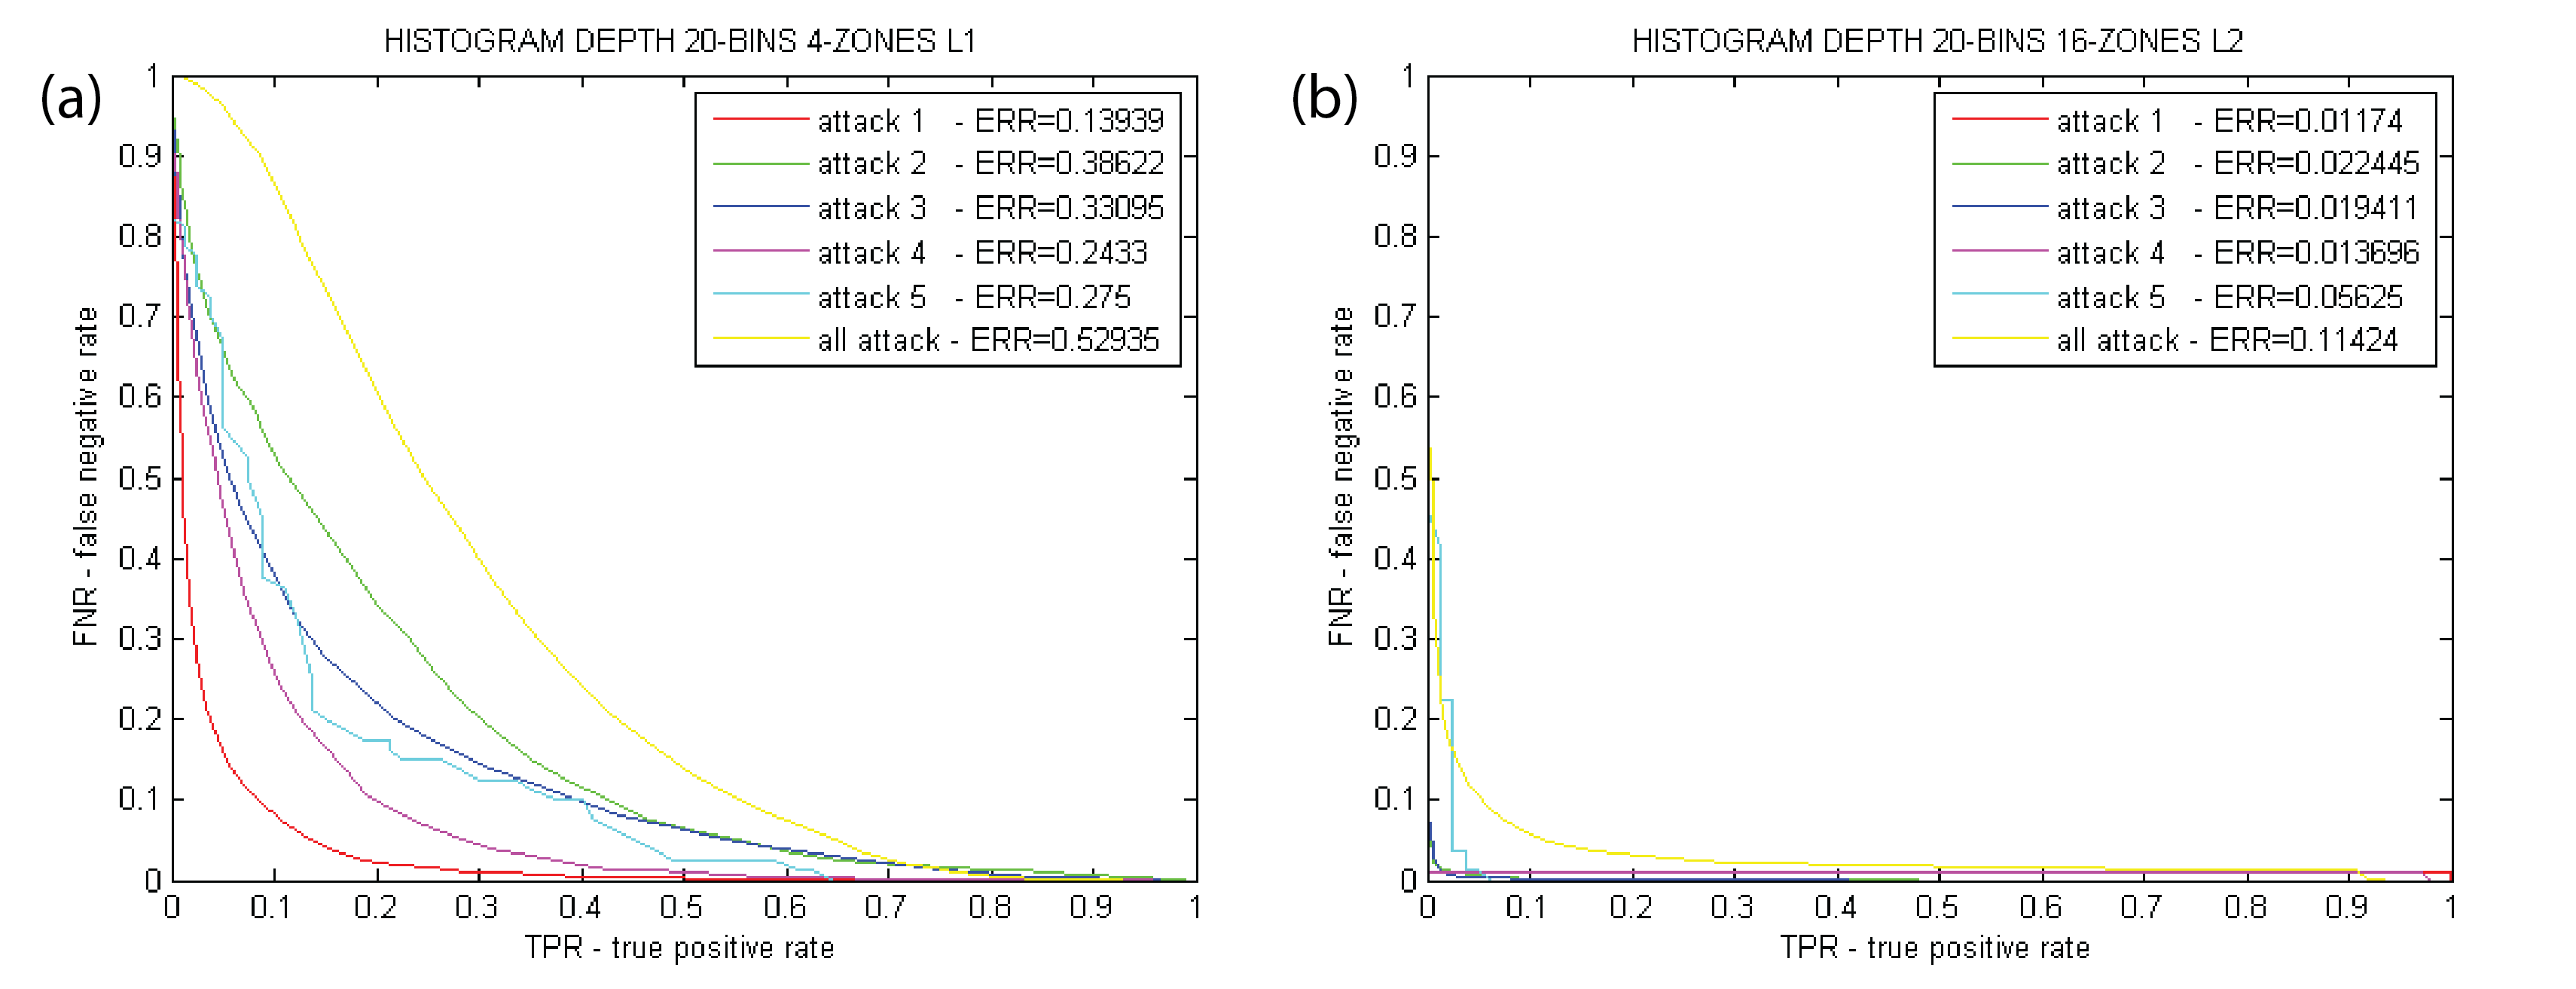
\includegraphics[width=1\textwidth]{ch-sistemasABC/images/ch-evaluacion_topologias/RESULTADOS_HISTOGRAMAS_POR_REGIONES.png}
    \caption{Resultados obtenidos al considerar histogramas por regiones para conservar la información local.}
    \label{fig:RESULTADOS_HISTOGRAMAS_POR_REGIONES}
\end{figure}

\paragraph{\textbf{Clasificación basada en la profundidad de los puntos \textit{landmark} de la cara}}.

Se calculan los \textit{landmark} de la cara con la librería \Gls{Dlib}.

Se crea un vector con las profundidades de los puntos (ver Fig- \ref{fig:LANDMARK_DETECTADOS}). 

\begin{figure}
\centering
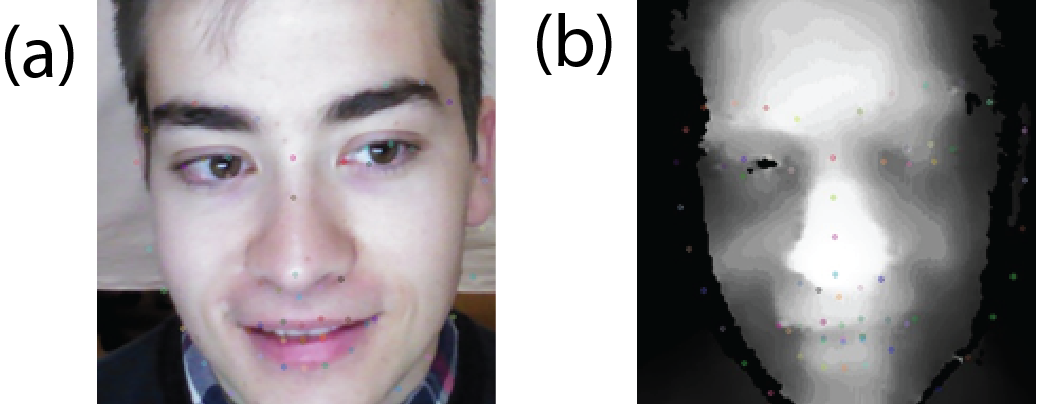
\includegraphics[width=1\textwidth]{ch-sistemasABC/images/ch-evaluacion_topologias/LANDMARK_DETECTADOS.png}
    \caption{\textit{landmark} faciales detectados.}
    \label{fig:LANDMARK_DETECTADOS}
\end{figure}

Se normaliza el vector de puntos (Se eliminan los \textit{outlayers} y se selecciona el máximo y el mínimo del vector CREO QUE ESTO NO ES CORRECTO DEBERÍA COGERSE LA MEDIA)

Los resultados obtenidos al considerar los \textit{landmark} son Fig. X. 

% \begin{figure}
% \centering
% 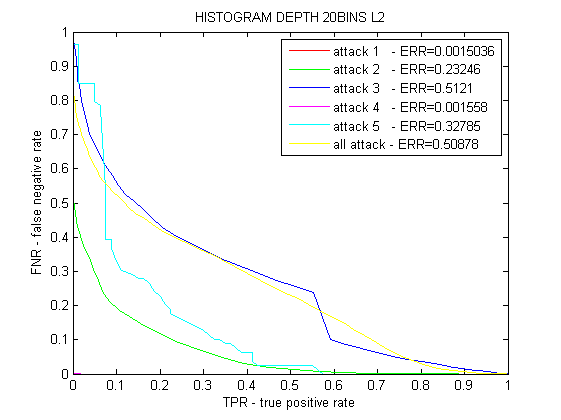
\includegraphics[width=1\textwidth]{ch-sistemasABC/images/ch-evaluacion_topologias/RESULTADOS_OPTENIDOS_CON_LANDMARK.png}
%     \caption{Resultados obtenidos considerando los \textit{landmark} de la cara.}
%     \label{fig:RESULTADOS_CON_LANDMARK}
% \end{figure}
